\documentclass[9pt,aspectratio=169]{beamer}


\usepackage{tabu, booktabs, multirow}
\usepackage{tabularx} 
\usepackage{multicol} 
\usepackage{setspace}
\usepackage[official]{eurosym}
\usepackage{graphicx}

\usepackage{hyperref}
\hypersetup{
    colorlinks=true,
    linkcolor=blue,
    filecolor=magenta,      
    urlcolor=cyan,
    pdftitle={EC3318/MN3101 Orientation Week 2026/27},
    pdfpagemode=FullScreen,
    }

\urlstyle{same}

\graphicspath{ {./pix_l0/} }



\newcolumntype{Y}{>{\centering\arraybackslash}X}  % Centered version of X

\newcommand{\placeholderbox}[1]{%
  \begin{center}
    \fbox{\parbox[c][0.5\textheight][c]{0.9\linewidth}{\centering \textit{#1}}}
  \end{center}
}
% St Andrews Color Palette

% Blues
\definecolor{StAndrewsLightBlue}{RGB}{0,174,239}
\definecolor{StAndrewsMidBlue}{RGB}{0,125,197}
\definecolor{StAndrewsBlue}{RGB}{0,83,155}  % Previously defined

% Reds
\definecolor{StAndrewsBurgundy}{RGB}{198,12,70}
\definecolor{StAndrewsRed}{RGB}{238,49,42}  % Previously defined

% Purple
\definecolor{StAndrewsPurple}{RGB}{123,67,154}

% Orange
\definecolor{StAndrewsOrange}{RGB}{245,132,43}

% Greens
\definecolor{StAndrewsGreen}{RGB}{84,185,72}
\definecolor{StAndrewsMidGreen}{RGB}{0,133,63}
\definecolor{StAndrewsDarkGreen}{RGB}{0,89,83}

% Yellow
\definecolor{StAndrewsYellow}{RGB}{255,223,0}

% Black
\definecolor{StAndrewsBlack}{RGB}{35,31,32}

\setbeamercolor*{structure}{fg=StAndrewsBlack}
\setbeamercolor{title}{fg=StAndrewsBlack}
\setbeamercolor{title separator}{fg=StAndrewsBlue}
\setbeamercolor{frametitle}{bg=StAndrewsBlue, fg=white}

\usetheme{metropolis}
\usepackage{tikz}
\usetikzlibrary{calc}
\usetikzlibrary{arrows.meta, positioning, shapes.geometric, shadows}
\usepackage[export]{adjustbox}
\usepackage{hyperref}
\hypersetup{
  colorlinks=true,
  linkcolor=StAndrewsBlue,
  urlcolor=StAndrewsBlue,
  citecolor=StAndrewsBlue
}

% Show a full-width colored header with title + subtitle
\setbeamercolor{frametitle}{bg=StAndrewsBlue, fg=white}
\setbeamercolor{framesubtitle}{fg=white}
\setbeamerfont{frametitle}{size=\Large,series=\mdseries}
\setbeamerfont{title}{series=\mdseries}
\setbeamerfont{framesubtitle}{size=\small}

\makeatletter
\setbeamertemplate{frametitle}{
  \nointerlineskip
  % Preserve the original header padding; ex changes slightly with font weight.
  \begin{beamercolorbox}[wd=\paperwidth,sep=4.6165pt,leftskip=1.2em,rightskip=1.2em]{frametitle}
    \usebeamerfont{frametitle}\strut\insertframetitle\par
    \ifx\insertframesubtitle\@empty\else
      \vspace{0.25ex}
      {\usebeamerfont{framesubtitle}\usebeamercolor[fg]{framesubtitle}\insertframesubtitle\par}
    \fi
  \end{beamercolorbox}
}
\makeatother

\makeatletter
\setbeamertemplate{title page}{
  \begin{minipage}[c][\textheight][c]{\textwidth}
    \centering
    \ifx\inserttitle\@empty\else\usebeamertemplate*{title}\fi
    \ifx\insertsubtitle\@empty\else\usebeamertemplate*{subtitle}\fi
    \vspace{8pt}
    {\usebeamercolor[fg]{title separator}\rule{0.72\textwidth}{0.4pt}\par}
    \vspace{10pt}
    \ifx\beamer@shortauthor\@empty\else\usebeamertemplate*{author}\fi
    \vspace{12pt}
    \ifx\insertinstitute\@empty\else\usebeamertemplate*{institute}\fi
    \vspace{6pt}
    \ifx\insertdate\@empty\else\usebeamertemplate*{date}\fi
    \vspace{9pt}
    \ifx\inserttitlegraphic\@empty\else\usebeamertemplate*{title graphic}\fi
  \end{minipage}
}

\setbeamertemplate{title}{
%  \raggedright%  % <-- Comment here
  \linespread{1.0}%
  \inserttitle%
  \par%
}
\setbeamertemplate{subtitle}{
%  \raggedright%  % <-- Comment here
  \insertsubtitle%
  \par%
  \vspace*{0.5em}
}
\setbeamertemplate{author}{
%  \raggedright%  % <-- Comment here
  \insertauthor%
  \par%
}
\setbeamertemplate{institute}{\insertinstitute\par}
\makeatother

\title{\LARGE Orientation Week lecture: \\
Corporate characteristics, management and control }
\author[Dr Christian Engels \& Dr Mao Zhang]{Dr Christian Engels}
\institute{\small{EC3318 Financial Economics: Corporate Finance \\ MN3101 Corporate Finance and Control \\[2mm] University of St Andrews Business School}}
\date{11 September 2026}


\newenvironment{wideitemize}{\itemize\addtolength{\itemsep}{10pt}}{\enditemize}
\setbeamertemplate{items}[circle]

\setbeamertemplate{title graphic}{\inserttitlegraphic\par}
\titlegraphic{
\includegraphics[scale=0.08]{logos/01-standard-black-text.png}}

% Add the logo to the bottom left
\addtobeamertemplate{footline}{%
  \begin{tikzpicture}[remember picture,overlay]
    \node[anchor=south west, inner sep=0pt] at ([xshift=0.5cm, yshift=0.25cm]current page.south west) {
      
\includegraphics[height=0.5cm]{logos/st-andrews-icon.png}
    };
  \end{tikzpicture}%
}{}

\begin{document}


\frame[plain]{\titlepage}


\begin{frame}{Content of today's Orientation Week lecture}
\begin{columns}[t]
  \begin{column}{0.29\textwidth}
    \tableofcontents[sections={1}]
  \end{column}
  \begin{column}{0.69\textwidth}
    \tableofcontents[sections={2}]
  \end{column}
\end{columns}
\end{frame}

\section[Part 1. Module overview]{\textbf{Part 1: Module overview}}

\subsection{Module content}

\begin{frame}{Welcome to learning Corporate Finance in EC3318/MN3101!}
\textbf{General points:}
\begin{itemize}
\item Shared teaching for EC3318 and MN3101; 20 credits in Semester 1, 2026/27.
  \item What this module is about: corporate financial decisions, governance, and value creation.  
  \item Who we are: \href{https://www.st-andrews.ac.uk/business-school/people/finance/ce50/}{Dr Christian Engels} (module coordinator) and \href{https://www.st-andrews.ac.uk/business-school/people/finance/mz71/}{Dr Mao Zhang}.
  \item Use your module's Moodle page for announcements, recordings and the reading list.
  \item Teaching: 20 lecture hours, two one-hour computational labs and three one-hour tutorials.
  \item \textbf{Orientation:} Fri 11 Sep, 9--10am, School III (UC0). \textbf{Lectures:} Tuesdays 4--6pm, Physics Lecture Theatre A (PHY), from 15 Sep 2026.
  \item In Moodle's \textbf{Before You Start}, select \textbf{Open the steps}: sign-up, calculator tagging and GitHub Education.
\end{itemize}
\end{frame}

\begin{frame}{Module learning outcomes}

\textbf{By the end of this module, students will be able to:}
\begin{itemize}
\item Explain corporate finance and the role of the financial manager.
\item Evaluate theories of corporate capital structure.
\item Understand the importance of discounted cash flow valuation.
\item Apply computational techniques to estimate securities' returns and risk.
\item Assess investment appraisal criteria.
\end{itemize}
\smallskip
{\footnotesize\href{https://www.st-andrews.ac.uk/subjects/modules/catalogue/?meta_semester_sand=1\&meta_modulecode=MN3101\&meta_ayrs_sand=2026\%2F7}{MN3101 module catalogue, 2026/27}, linked from Moodle.\par}

\end{frame}

\subsection{Semester schedule}

\begin{frame}{Module timing: Semester 1, 2026/27}
\begingroup
\renewcommand{\arraystretch}{1.0}
\setlength{\tabcolsep}{3pt}
\begin{tabularx}{\textwidth}{@{}l l >{\raggedright\arraybackslash}X l@{}}
\toprule
\textbf{Week} & \textbf{Week commencing} & \textbf{Topic} & \textbf{Session} \\
\midrule
Orientation & 7 Sep & Corporate characteristics, management and control & \\
1 & 14 Sep & Discounting, compounding and investment appraisal & \\
2 & 21 Sep & Discount factors and cost of capital & Lab \\
3 & 28 Sep & Valuation models: stocks and bonds & \\
4 & 5 Oct & Capital structure: perfect/imperfect markets & Lab \\
5 & 12 Oct & Class test & 13 Oct \\
6 & 19 Oct & Independent Learning Week & \\
7 & 26 Oct & Payout policy: perfect/imperfect markets & Tutorial \\
8 & 2 Nov & Equity funding and IPOs & \\
9 & 9 Nov & Mergers & Tutorial \\
10 & 16 Nov & Sustainable corporate finance & \\
11 & 23 Nov & Revision & Tutorial \\
12 & 30 Nov & University revision week: no new teaching & \\
\bottomrule
\end{tabularx}
\endgroup
\end{frame}

\subsection{Assessments}

\begin{frame}{Assessments overview}
\renewcommand{\arraystretch}{1.5}
\begin{table}[h!]
\centering
\begin{tabularx}{\textwidth}{l c X}
\hline
\textbf{Assessment} & \textbf{Weight (\%)} & \textbf{Date / deadline (2026)} \\
\hline
Class Test & 25 & Tue 13 October, 4--5pm (Week 5); in person, replacing the lecture \\
Technical Assignment & 25 & Fri 13 November, 12 noon (Week 9); submit through MMS \\
Final Exam & 50 & December examination diet; in person, exact date to be confirmed centrally \\
\hline
\end{tabularx}
\end{table}
\end{frame}

\begin{frame}{Assessments details}
\begin{columns}[T,onlytextwidth]
\begin{column}{0.45\textwidth}
\textcolor{StAndrewsBlue}{\textbf{Class test (25\%)}}
\begin{itemize}
    \item In person; replaces the scheduled lecture.
    \item \textbf{AI Level 1: no AI} at any point during the assessment.
\end{itemize}
\medskip
\textcolor{StAndrewsBlue}{\textbf{Final exam (50\%)}}
\begin{itemize}
    \item In person; date set centrally.
    \item Check Moodle for the current assessment instructions.
\end{itemize}
\end{column}
\begin{column}{0.49\textwidth}
\textcolor{StAndrewsBlue}{\textbf{Technical assignment (25\%)}}
\begin{itemize}
    \item \textbf{AI Level 5:} coding, empirical output, tables and figures. You must check and explain the work.
    \item \textbf{AI Level 3:} edit your own writing; AI must not create new written content.
    \item Complete the required AI declaration and cite AI-created content (tools/prompts where required). Coversheet on Moodle.
\end{itemize}
\end{column}
\end{columns}
\vspace{0.7em}
\textbf{Calculator:} University-approved and tagged for class tests/exams. Tagging at Gateway Reception: bring your calculator and student ID; no booking needed.
\par\smallskip
{\footnotesize See \textbf{Assessments} and \textbf{Before you start} on Moodle for the full requirements.\par}
\end{frame}

\subsection{Tutorials and labs}

\begin{frame}{Tutorial and Lab sign-up on MMS}

\textbf{Please note these important points:}
\begin{itemize}
  \item Opens \textbf{Mon 14 Sep, 12 noon}; closes \textbf{Mon 28 Sep, 12 noon} (2026, Weeks 1 and 3).
  \item You must sign up for \alert{both a \emph{tutorial} and a \emph{lab}} (not one or the other).
  \item Attendance is required. Check your timetable across \emph{all relevant weeks} before choosing to avoid clashes.
  \item Places are limited; if a group is full, please choose an alternative.
  \item If you do not sign up by the deadline, you will be \textbf{automatically assigned} to a group with space.
\end{itemize}

\vspace{0.5em}
\textbf{When sessions run}

\begin{tabular}{@{}ll@{}}
Labs: & Weeks 2 and 4 \\
Tutorials: & Weeks 7, 9 and 11 \\
\end{tabular}

\vspace{0.6em}
\textbf{Administration:} use Moodle's guidance first; unresolved sign-up queries:

\begin{tabular}{@{}ll@{}}
EC3318: & \href{mailto:econadmin@st-andrews.ac.uk}{econadmin@st-andrews.ac.uk}  \\
MN3101: & \href{mailto:manug@st-andrews.ac.uk}{manug@st-andrews.ac.uk}  \\
\end{tabular}
\end{frame}

\subsection{References}

\begin{frame}{Main references}

\textbf{Textbooks:}

Hillier, D., Ross, S., Westerfield, R., Jaffe, J. \& Jordan, B. (2021) Corporate Finance. 4th ed.
London: McGraw-Hill Education. ISBN-13: 9781526848086.

Brealey, R. A., Myers, S. C., Allen, F., \& Edmans, A. (2022). Principles of Corporate Finance (14th ed.). McGraw-Hill Education. ISBN: 978-1265074159.

\textbf{Prepare for the labs:}

Create a GitHub account using your \texttt{@st-andrews.ac.uk} email and apply for GitHub Education \textbf{as soon as possible}. Bring a working login to the lab. Follow Moodle's \textbf{Before you start} steps.

\textbf{Python resources:}

Scheuch, Voigt, Weiss \& Frey (2024), \href{https://www.tidy-finance.org/python/}{\textit{Tidy Finance with Python}}.

Software Carpentry: \href{https://swcarpentry.github.io/python-novice-inflammation/}{Programming with Python}; \href{https://swcarpentry.github.io/python-novice-gapminder}{Plotting and programming with Python}.

\textbf{Each week:} consult your Moodle reading list and the required/further reading.
    
\end{frame}

\begin{frame}{Questions remaining? Follow the module's help route}
First review the materials we have supplied: slides, readings, recordings, Moodle guidance and announcements.
\par\medskip
\textcolor{StAndrewsBurgundy}{\textbf{Still have a question? Office hours $\rightarrow$ email}}
\par\medskip
\begin{columns}[T,onlytextwidth]
\begin{column}{0.46\textwidth}
\textcolor{StAndrewsBlue}{\textbf{1. Office hours}}\par
Use the booking details in Moodle's \textbf{Contacts}. Bring the point where you got stuck.
\end{column}
\begin{column}{0.46\textwidth}
\textcolor{StAndrewsBlue}{\textbf{2. Email}}\par
Only if your query remains unresolved after office hours. Explain what you have checked and tried.
\end{column}
\end{columns}
\par\medskip
\textbf{Absent or missing an assessment?} Follow your module's self-certification / extenuating-circumstances procedure. No separate message to the teaching team is needed alongside the forms.
  
\end{frame}

% Part B additions use the existing theme and typography.
\newcommand{\partbsource}[1]{\par\vspace{0.5em}{\footnotesize #1\par}}
% Shared styles; the lecture already loads fontspec and TikZ.
\providecolor{StAndrewsBlue}{HTML}{00539B}
\providecolor{StAndrewsBurgundy}{HTML}{C60C46}
\providecolor{DiagramInk}{HTML}{231F20}
\providecolor{DiagramPaper}{HTML}{FAFAFA}
\newfontfamily\DiagramFira{Fira Sans}
\tikzset{
 diagram/.style={x=1pt,y=1pt,font=\DiagramFira\linespread{1}\fontsize{9}{11}\selectfont,text=DiagramInk},
 diagram box/.style={rectangle,draw=StAndrewsBlue,line width=.6pt,fill=DiagramPaper,inner sep=4pt,outer sep=0pt,align=center},
 diagram blue/.style={diagram box,fill=StAndrewsBlue,text=white},
 diagram burgundy/.style={diagram box,draw=StAndrewsBurgundy,text=StAndrewsBurgundy},
 diagram label/.style={rectangle,inner sep=0pt,outer sep=0pt,align=center},
 diagram edge/.style={draw=StAndrewsBlue,line width=.8pt,line cap=butt,line join=miter},
 diagram forward/.style={diagram edge,-{Triangle[length=4pt,width=4pt]}},
 diagram both/.style={diagram edge,{Triangle[length=4pt,width=4pt]}-{Triangle[length=4pt,width=4pt]}},
 diagram cash/.style={diagram forward,draw=StAndrewsBurgundy}
}
\newif\ifDiagramAudit
\newif\ifDiagramDebug
\newwrite\DiagramCSV
\makeatletter
\newcommand{\DiagramMeasure}[3]{%
 \ifDiagramAudit
  \pgfextractx{\dimen0}{\pgfpointanchor{#2}{south west}}%
  \pgfextracty{\dimen2}{\pgfpointanchor{#2}{south west}}%
  \pgfextractx{\dimen4}{\pgfpointanchor{#2}{north east}}%
  \pgfextracty{\dimen6}{\pgfpointanchor{#2}{north east}}%
  \immediate\write\DiagramCSV{#1,#2,#3,\strip@pt\dimen0,\strip@pt\dimen2,\strip@pt\dimen4,\strip@pt\dimen6}%
 \fi
 \ifDiagramDebug
  \draw[red,line width=.2pt] (#2.south west) rectangle (#2.north east);
 \fi
}
\makeatother


\section[Part 2: Corporate characteristics, management and control]{\textbf{Part 2: Corporate characteristics, management and control}}

\begin{frame}{Topics covered} 
\begin{wideitemize}
    \item The Concept of Corporate Finance
\item Forms of Business Organisation
\item Corporate Finance Decisions
\item The Goal of Corporate Finance Decisions
\item Financial Markets and the Corporation
\end{wideitemize}

\end{frame}


% (PDF p.3) Reading
\begin{frame}{Required reading}
\begin{enumerate}
\item Hillier, D., Ross, S., Westerfield, R., Jaffe, J. and Jordan, B. (2021)
Corporate Finance. 4th ed. Chapter 1.
\item  Brealey, R. A., Myers, S. C., Allen, F., \& Edmans, A. (2022). Principles of Corporate Finance (14th ed.). McGraw-Hill Education. ISBN: 978-1265074159. Chapter 1.
\item  La Porta, R., Lopez-de-Silanes, F. and Shleifer, A. (1999) Corporate
Ownership Around the World. Journal of Finance 54, 471-517.
\href{https://doi.org/10.1111/0022-1082.00115}{https://doi.org/10.1111/0022-1082.00115}
\item  Zingales, L. (2015) Presidential Address: Does Finance Benefit
Society? Journal of Finance 70, 1327-1363.
\href{https://doi.org/10.1111/jofi.12295}{https://doi.org/10.1111/jofi.12295}
\end{enumerate}
\end{frame}

\subsection{What is Corporate Finance?}
% (PDF p.4) What is Corporate Finance?
\begin{frame}{What is Corporate Finance?}
\begin{columns}[T,onlytextwidth]
\begin{column}{0.30\textwidth}
\textcolor{StAndrewsBlue}{\textbf{Investment}}\par\smallskip
Which assets and projects should the firm invest in?
\end{column}
\begin{column}{0.30\textwidth}
\textcolor{StAndrewsBlue}{\textbf{Financing}}\par\smallskip
How should it fund those investments?
\end{column}
\begin{column}{0.30\textwidth}
\textcolor{StAndrewsBlue}{\textbf{Working capital}}\par\smallskip
How should it manage short-term assets and liabilities?
\end{column}
\end{columns}
\vspace{1.4em}
These choices determine the \textbf{magnitude, timing and risk} of cash flows.
\par\vspace{0.8em}
\textcolor{StAndrewsBlue}{\rule{\textwidth}{0.4pt}}\par\smallskip
\textbf{Governance:} who makes these decisions, and in whose interests?
\partbsource{These are the three financial decisions developed below; see the Chapter 1 readings.}
\end{frame}

\subsection{Forms of business organisation}
% (PDF p.5) Sole Trader
\begin{frame}{Forms of Business Organisation: Sole Trader}
\begin{wideitemize}
\item Owned and run by one person; straightforward to establish.
\item Profits are subject to the owner's income tax, rather than corporation tax.
\item \textbf{Unlimited liability:} the owner is personally responsible for business debts.
\item Business assets can be sold, but there are no company shares to transfer.
\item Can use personal funds and borrow; cannot raise equity by issuing shares.
\end{wideitemize}
\partbsource{UK context: \href{https://www.gov.uk/become-sole-trader}{GOV.UK, sole traders}.}
\end{frame}

% (PDF p.6) Partnership
\begin{frame}{Forms of Business Organisation: Partnership}
\begin{wideitemize}
\item An \textbf{ordinary partnership} is a business carried on by two or more partners.
\item Partners share profits and responsibility for the business.
\item Partners are taxed on their shares of profit; partners can be individuals or companies.
\item Management, changes in membership and continuity depend on the agreement and the law.
\item In Scotland, the partnership has separate legal personality; partners can still be personally liable for its debts.
\end{wideitemize}
\partbsource{\href{https://www.gov.uk/set-up-business-partnership}{GOV.UK, partnerships}; \href{https://www.gov.uk/hmrc-internal-manuals/vat-registration-manual/vatreg09050}{HMRC, partnerships in Scotland}.}
\end{frame}

% (PDF p.7) Types of Partnership
\begin{frame}{Partnership Types}
\begingroup
\renewcommand{\arraystretch}{1.3}
\begin{tabularx}{\textwidth}{@{}>{\raggedright\arraybackslash}p{0.28\textwidth}>{\raggedright\arraybackslash}X@{}}
\textcolor{StAndrewsBlue}{\textbf{Ordinary partnership}} & Partners have unlimited personal liability. \\[0.5em]
\textcolor{StAndrewsBlue}{\textbf{Limited partnership}} & General partners manage and have unlimited liability; limited partners normally risk their contribution and do not manage. \\[0.5em]
\textcolor{StAndrewsBlue}{\textbf{Limited liability partnership (LLP)}} & A separate body corporate; members' liability is generally limited. \\
\end{tabularx}
\endgroup
\par\vspace{0.6em}
Partners and members can be individuals or companies.
\par\vspace{0.5em}
\textbf{US distinction:} a limited liability company (LLC) is a distinct state-law form, with several possible tax classifications.
\partbsource{\href{https://www.gov.uk/guidance/set-up-and-run-a-limited-liability-partnership-llp}{GOV.UK, LLPs}; \href{https://www.gov.uk/guidance/set-up-and-run-a-limited-partnership}{limited partnerships}; \href{https://www.irs.gov/businesses/small-businesses-self-employed/limited-liability-company-llc}{IRS, LLCs}.}
\end{frame}

\subsection{Real life company examples}

% (PDF p.8) PwC LLP (image-heavy)
\begin{frame}{Example: PricewaterhouseCoopers (UK) LLP}
\begin{multicols}{2}
\begin{itemize}
\item UK LLP: a member firm in the PwC global network.
\item \textbf{Global network, FY2025:} 136 countries; US\$56.9bn revenue.
\item \textbf{UK consolidated group, FY2025:} £6.35bn revenue; includes Middle East and Channel Islands businesses.
\item \textbf{UK partners, FY2025:} average distributable profit of £865,000 per partner.
\end{itemize}

\columnbreak


\includegraphics[scale=0.3]{pwc.png}
\end{multicols}
\partbsource{\href{https://www.pwc.com/gx/en/about/global-annual-review/financial-performance.html}{PwC Global Annual Review 2025}; \href{https://www.pwc.co.uk/press-room/press-releases/corporate-news/2025-financial-results-resilience-in-a-year-of-transformation-and-change.html}{PwC UK 2025 financial results}. Figures cover different entities.}
\end{frame}

% (PDF p.9) Soros Fund Management LLC (image-heavy)
\begin{frame}{Example: Soros Fund Management LLC (2011)}
\begin{multicols}{2}
\begin{itemize}
\item In 2011, Soros Fund Management announced it would return outside capital and operate as a family office.
\item The Dodd--Frank Act (2010) removed the former private-adviser exemption.
\item The SEC's 2011 family-office rule excludes qualifying family-only, family-owned and controlled offices from investment-adviser registration.
\item Changing the client boundary changed its regulatory position.
\end{itemize}

\columnbreak

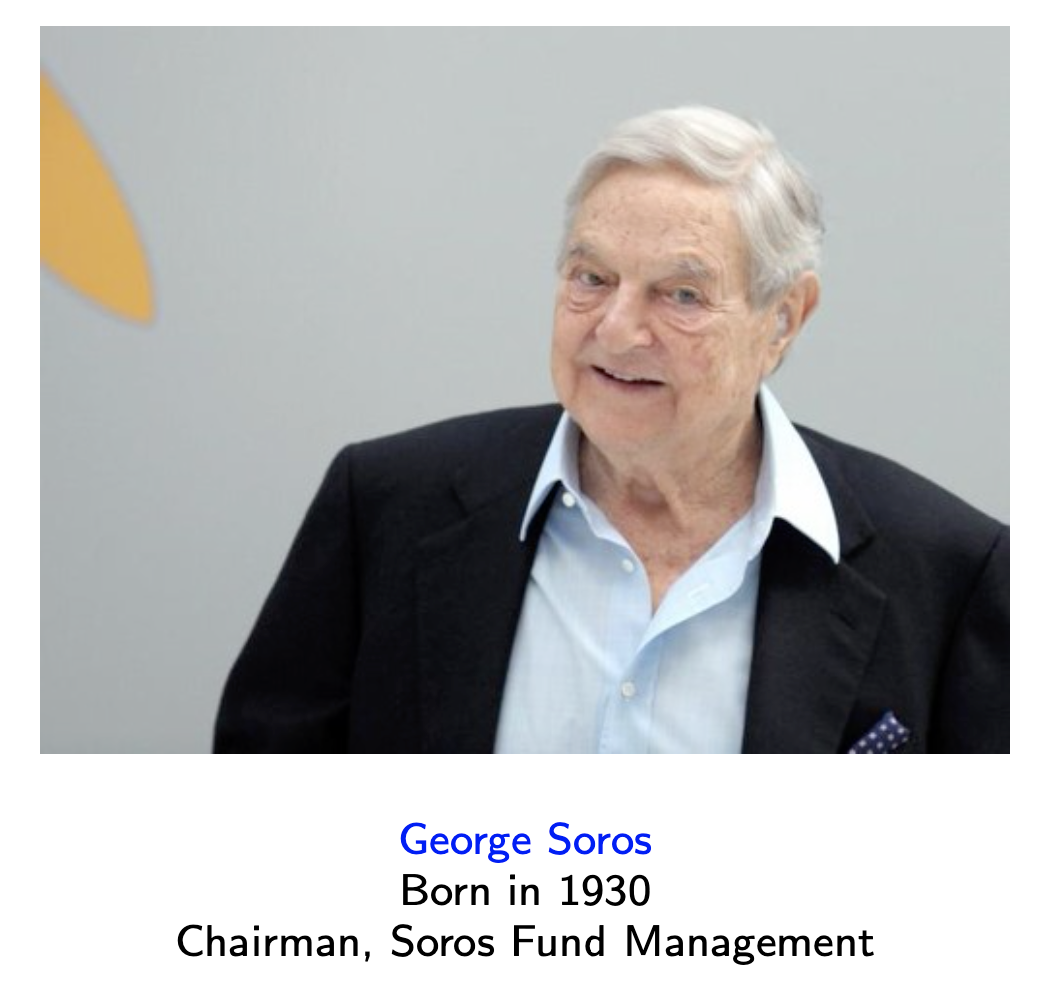
\includegraphics[scale=0.3]{george_soros.png}
\end{multicols}
\partbsource{\href{https://media.ft.com/cms/e11bf598-b780-11e0-b95d-00144feabdc0.pdf}{Soros investor letter, July 2011}; \href{https://www.sec.gov/news/press/2011/2011-134.htm}{SEC family-office rule, June 2011}. Other legal obligations still apply.}
\end{frame}

\subsection{Corporations}

% (PDF p.10) Corporation
\begin{frame}{Corporations}
\begin{wideitemize}
\item Here we focus on \textbf{companies limited by shares}, owned by one or more shareholders.
\item The company is a separate legal person, with its own assets and debts.
\item Shareholders' liability is generally limited to any unpaid amount on their shares.
\item Company profits are subject to corporation tax; distributions may also be taxed.
\item \textbf{Private/public} describes legal status, not the number of shareholders. Private companies cannot offer their shares to the public.
\end{wideitemize}
\partbsource{UK context: \href{https://www.gov.uk/limited-company-formation}{GOV.UK, limited companies}; Companies Act 2006, ss.3, 4 and 755.}
\end{frame}

% (PDF p.11) Public Corporation
\begin{frame}{Public Corporations}
\begin{wideitemize}
\item A public company can be \textbf{listed or unlisted}.
\item Listed shares trade on stock exchanges, making ownership easier to transfer.
\item The company can continue when shareholders change or die.
\item Shareholders elect a board; managers take day-to-day decisions.
\item Ownership may be dispersed or concentrated: a listed firm can still have a controlling shareholder.
\item Listed companies face additional disclosure and market rules.
\end{wideitemize}
\partbsource{Ownership and control: \href{https://doi.org/10.1111/0022-1082.00115}{La Porta, Lopez-de-Silanes and Shleifer (1999)}.}
\end{frame}

% Updated example: economic ownership and voting control.
\begin{frame}{Ownership example: Meta}
\textbf{Mark Zuckerberg's economic interest and voting power}
\par\begingroup\centering
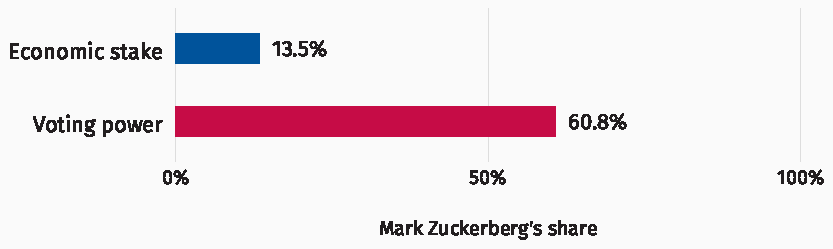
\includegraphics[width=\textwidth,height=0.62\textheight,keepaspectratio]{figures/meta_control.pdf}
\par\endgroup
Class A shares carry one vote; Class B shares carry ten.\\
\textbf{For reflection:} Can someone control a company without owning most of its shares?
\partbsource{\href{https://www.sec.gov/Archives/edgar/data/1326801/000162828026025532/meta-20260416.htm}{Meta 2026 proxy, pp.63--64}, holdings at 1 April 2026. Economic interest calculated from share counts.\\
Dual-class governance: \href{https://doi.org/10.1093/rfs/hhp024}{Gompers, Ishii and Metrick (2010)}.}
\end{frame}

% (PDF p.16) Summary (end of Part 1 block)
\begin{frame}{Summary: Business Organisations}
\begingroup
\renewcommand{\arraystretch}{1.35}
\setlength{\tabcolsep}{4pt}
\begin{tabularx}{\textwidth}{@{}l>{\raggedright\arraybackslash}X>{\raggedright\arraybackslash}X>{\raggedright\arraybackslash}X@{}}
\toprule
\textbf{Form} & \textbf{Personal liability} & \textbf{Who decides?} & \textbf{Funding access} \\
\midrule
Sole trader & Owner liable & Owner & Own funds; borrowing \\
Ordinary partnership & Partners liable & Partners & Partner capital; borrowing \\
Limited partnership & General: unlimited; limited: contribution at risk & General partners & Partner capital; borrowing \\
LLP & Generally limited & Members' agreement & Member capital; borrowing \\
Company limited by shares & Generally limited & Board; shareholder votes & Share capital; borrowing \\
\bottomrule
\end{tabularx}
\endgroup
\partbsource{Public/private legal status and listed/unlisted market status are separate.\\
\href{https://doi.org/10.2307/797521}{Hansmann and Kraakman (2000)}; UK qualifications and official sources in the accompanying source notes.}
\end{frame}

\begin{frame}{Most UK businesses are sole proprietorships}
\textbf{5.69 million private-sector businesses at the start of 2025}
\par\begingroup\centering
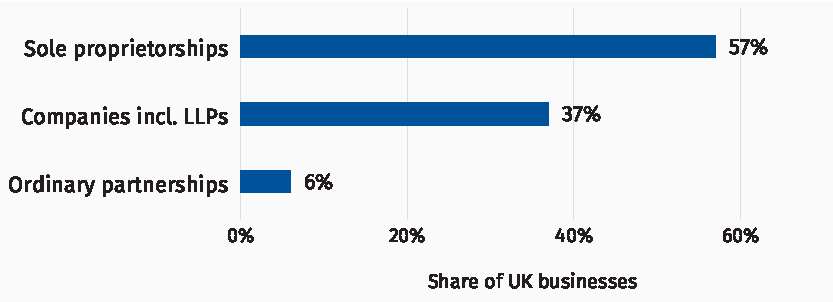
\includegraphics[width=\textwidth,height=0.59\textheight,keepaspectratio]{figures/uk_business_forms.pdf}
\par\endgroup
\textbf{For reflection:} Does the most common form necessarily account for the most output?
\partbsource{\href{https://www.gov.uk/government/statistics/business-population-estimates-2025/business-population-estimates-for-the-uk-and-regions-2025-statistical-release}{DBT, Business Population Estimates 2025}, Figure 5. Shares of businesses by count, rounded.\\
Includes estimated unregistered businesses; DBT's companies category includes LLPs.}
\end{frame}

\subsection{Financial management decisions}

% (PDF p.17) Financial Management Decisions
\begin{frame}{Financial Management Decisions}
\centering
% Coordinate map: TeX pt, origin lower left; fixed canvas x=0..390, y=0..165.
% Edit nodes/routes here. The build script reads these commands and audit metadata.
\begin{tikzpicture}[diagram]
% audit-node {"id":"questions","kind":"box","text":"Financial decisions","parent":null,"padding":4,"outline_width":0.6}
\node[diagram blue,minimum width=124pt,minimum height=24pt] (questions) at (195,145) {Financial decisions};
% audit-node {"id":"investment-q","kind":"box","text":"What to do with the money","parent":null,"padding":4,"outline_width":0.6}
\node[diagram blue,minimum width=116pt,minimum height=34pt] (investment-q) at (64,91) {What to do with\\the money};
% audit-node {"id":"financing-q","kind":"box","text":"Where to get the money","parent":null,"padding":4,"outline_width":0.6}
\node[diagram blue,minimum width=116pt,minimum height=34pt] (financing-q) at (195,91) {Where to get\\the money};
% audit-node {"id":"liquidity-q","kind":"box","text":"How to stay liquid","parent":null,"padding":4,"outline_width":0.6}
\node[diagram blue,minimum width=116pt,minimum height=34pt] (liquidity-q) at (326,91) {How to stay\\liquid};
% audit-node {"id":"investment","kind":"box","text":"Investment Capital budgeting","parent":null,"padding":4,"outline_width":0.6}
\node[diagram box,minimum width=116pt,minimum height=36pt] (investment) at (64,27) {Investment\\Capital budgeting};
% audit-node {"id":"financing","kind":"box","text":"Financing Capital structure","parent":null,"padding":4,"outline_width":0.6}
\node[diagram box,minimum width=116pt,minimum height=36pt] (financing) at (195,27) {Financing\\Capital structure};
% audit-node {"id":"liquidity","kind":"box","text":"Liquidity Working capital","parent":null,"padding":4,"outline_width":0.6}
\node[diagram box,minimum width=116pt,minimum height=36pt] (liquidity) at (326,27) {Liquidity\\Working capital};
% audit-route {"id":"q-invest","source":"questions","target":"investment-q","arrow":"target","shared_junctions":[],"outline_width":0.8,"arrow_length":4,"arrow_width":4}
\draw[diagram forward] (155,130) -- (64,130) -- (64,111);
% audit-route {"id":"q-finance","source":"questions","target":"financing-q","arrow":"target","shared_junctions":[],"outline_width":0.8,"arrow_length":4,"arrow_width":4}
\draw[diagram forward] (195,130) -- (195,111);
% audit-route {"id":"q-liquid","source":"questions","target":"liquidity-q","arrow":"target","shared_junctions":[],"outline_width":0.8,"arrow_length":4,"arrow_width":4}
\draw[diagram forward] (235,130) -- (326,130) -- (326,111);
% audit-route {"id":"investment-link","source":"investment-q","target":"investment","arrow":"target","shared_junctions":[],"outline_width":0.8,"arrow_length":4,"arrow_width":4}
\draw[diagram forward] (64,71) -- (64,48);
% audit-route {"id":"financing-link","source":"financing-q","target":"financing","arrow":"target","shared_junctions":[],"outline_width":0.8,"arrow_length":4,"arrow_width":4}
\draw[diagram forward] (195,71) -- (195,48);
% audit-route {"id":"liquidity-link","source":"liquidity-q","target":"liquidity","arrow":"target","shared_junctions":[],"outline_width":0.8,"arrow_length":4,"arrow_width":4}
\draw[diagram forward] (326,71) -- (326,48);
\DiagramMeasure{financial_management_decisions}{questions}{box}
\DiagramMeasure{financial_management_decisions}{investment-q}{box}
\DiagramMeasure{financial_management_decisions}{financing-q}{box}
\DiagramMeasure{financial_management_decisions}{liquidity-q}{box}
\DiagramMeasure{financial_management_decisions}{investment}{box}
\DiagramMeasure{financial_management_decisions}{financing}{box}
\DiagramMeasure{financial_management_decisions}{liquidity}{box}
\pgfresetboundingbox
\path[use as bounding box] (0,0) rectangle (390,165);
\end{tikzpicture}


\end{frame}

% (PDF p.18) Capital Budgeting
\begin{frame}{Capital Budgeting}
\par\begingroup\centering
{\Large\textcolor{StAndrewsBlue}{Which long-term projects should the firm undertake?}\par}
\smallskip
Plan and manage investments through cost–benefit analysis.
\par\endgroup
\vspace{1.8em}
\textbf{Evaluate the cash flows along three dimensions:}
\par\vspace{0.8em}
\begin{columns}[T,onlytextwidth]
\begin{column}{0.30\textwidth}
\textcolor{StAndrewsBlue}{\textbf{Magnitude}}\par\smallskip
How much comes in and goes out?
\end{column}
\begin{column}{0.30\textwidth}
\textcolor{StAndrewsBlue}{\textbf{Timing}}\par\smallskip
When do the cash flows occur?
\end{column}
\begin{column}{0.30\textwidth}
\textcolor{StAndrewsBlue}{\textbf{Risk}}\par\smallskip
Which outcomes are possible, and with what probabilities?
\end{column}
\end{columns}
\end{frame}

\begin{frame}{Firms use several methods to appraise investments}
\textbf{NPV:} value today of project cash flows, less its cost.\\
\textbf{Payback:} time needed to recover the initial investment.
\par\begingroup\centering
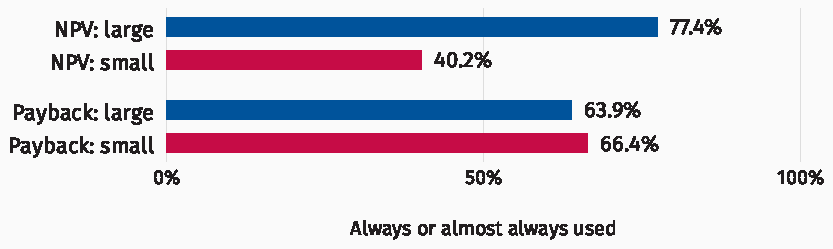
\includegraphics[width=\textwidth,height=0.56\textheight,keepaspectratio]{figures/cfo_practice.pdf}
\par\endgroup
\textbf{For reflection:} Why might a firm use both methods?
\partbsource{\href{https://doi.org/10.1111/jofi.13161}{Graham (2022)}, Table I, Panel A: March 2020 survey; always/almost always used.\\
Large/small firms: revenue above/below US\$1bn; multiple methods may be used.}
\end{frame}

% (PDF p.19) Capital Structure
\begin{frame}{Capital Structure}
\begin{wideitemize}
  \item Mix of debt (contractual claims) and equity (residual ownership claims).
  \item Short- vs long-term debt.
  \item How much should the firm borrow? Balance funding costs with financial risk.
  \item Raising capital: where, how, and when?
\end{wideitemize}
\end{frame}

% (PDF p.20) Working Capital
\begin{frame}{Working Capital Management}
\begin{wideitemize}
\item The management of short-term assets and liabilities
\item How much cash and inventory should be on hand?
\item Sell on credit? If so, on what terms and to whom?
\item How can short-term financing be obtained?
\end{wideitemize}
\end{frame}

\begin{frame}{The Interlocking Relationship}
\centering
% Coordinate map: TeX pt, origin lower left; fixed canvas x=0..390, y=0..165.
% Edit nodes/routes here. The build script reads these commands and audit metadata.
\begin{tikzpicture}[diagram]
% audit-node {"id":"budgeting","kind":"box","text":"Capital budgeting Investment choices","parent":null,"padding":4,"outline_width":0.6}
\node[diagram blue,minimum width=132pt,minimum height=40pt] (budgeting) at (195,132) {Capital budgeting\\Investment choices};
% audit-node {"id":"structure","kind":"box","text":"Capital structure Funding choices","parent":null,"padding":4,"outline_width":0.6}
\node[diagram blue,minimum width=136pt,minimum height=40pt] (structure) at (81,35) {Capital structure\\Funding choices};
% audit-node {"id":"working","kind":"box","text":"Working capital Liquidity choices","parent":null,"padding":4,"outline_width":0.6}
\node[diagram blue,minimum width=136pt,minimum height=40pt] (working) at (309,35) {Working capital\\Liquidity choices};
% audit-route {"id":"budget-structure","source":"budgeting","target":"structure","arrow":"both","shared_junctions":[],"outline_width":0.8,"arrow_length":4,"arrow_width":4}
\draw[diagram both] (160,109) -- (102,58);
% audit-route {"id":"budget-working","source":"budgeting","target":"working","arrow":"both","shared_junctions":[],"outline_width":0.8,"arrow_length":4,"arrow_width":4}
\draw[diagram both] (230,109) -- (288,58);
% audit-route {"id":"structure-working","source":"structure","target":"working","arrow":"both","shared_junctions":[],"outline_width":0.8,"arrow_length":4,"arrow_width":4}
\draw[diagram both] (152,35) -- (238,35);
\DiagramMeasure{interlocking_relationship}{budgeting}{box}
\DiagramMeasure{interlocking_relationship}{structure}{box}
\DiagramMeasure{interlocking_relationship}{working}{box}
\pgfresetboundingbox
\path[use as bounding box] (0,0) rectangle (390,165);
\end{tikzpicture}


\end{frame}

% (PDF p.22) Northern Rock (case)
\begin{frame}{Case: Northern Rock}
\begin{columns}[c,onlytextwidth]
\begin{column}{0.64\textwidth}
\begingroup
\renewcommand{\arraystretch}{1.2}
\setlength{\tabcolsep}{3pt}
\begin{tabularx}{\linewidth}{@{}>{\raggedright\arraybackslash}p{0.22\linewidth}>{\raggedright\arraybackslash}X@{}}
\textcolor{StAndrewsBlue}{\textbf{1997}} & Demutualised and became a listed bank. \\[0.45em]
\textcolor{StAndrewsBlue}{\textbf{Aug 2007}} & Wholesale-market disruption made refinancing difficult. \\[0.45em]
\textcolor{StAndrewsBlue}{\textbf{Sep 2007}} & Bank of England support became public; depositors queued to withdraw funds. \\[0.45em]
\textcolor{StAndrewsBlue}{\textbf{2008}} & Public ownership. \\[0.45em]
\textcolor{StAndrewsBlue}{\textbf{Jan 2012}} & Sale to Virgin Money completed. \\
\end{tabularx}
\endgroup
\end{column}
\begin{column}{0.31\textwidth}
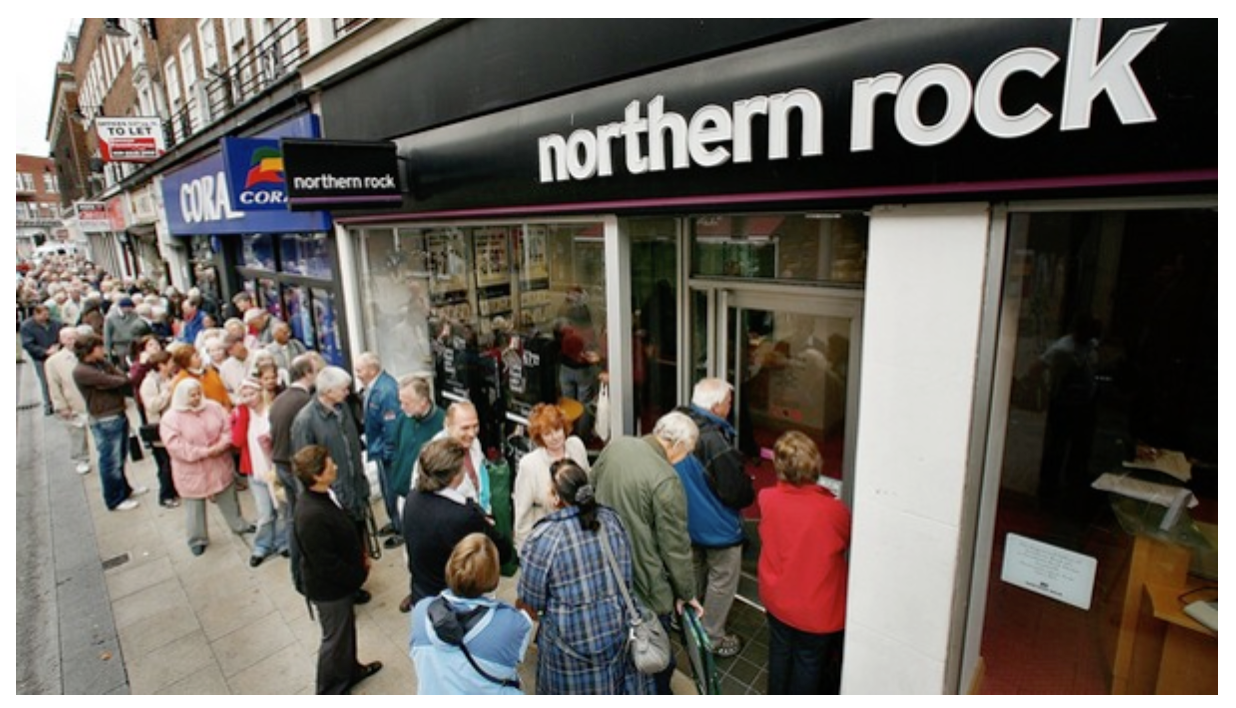
\includegraphics[width=\linewidth]{northern_rock.png}
\end{column}
\end{columns}
\partbsource{\href{https://doi.org/10.1257/jep.23.1.101}{Shin (2009)}; \href{https://www.nao.org.uk/reports/the-creation-and-sale-of-northern-rock-plc/}{NAO (2012)}. The funding disruption preceded the visible depositor run.}
\end{frame}

\begin{frame}{Bank of England lending replaced lost funding}
\par\begingroup\centering
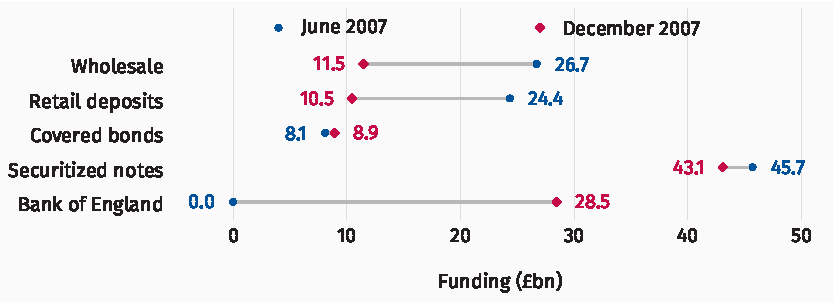
\includegraphics[width=\textwidth,height=0.66\textheight,keepaspectratio]{figures/northern_rock_funding.pdf}
\par\endgroup
\textbf{For reflection:} What happens when long-term assets depend on funding that must be renewed?
\partbsource{\href{https://doi.org/10.1257/jep.23.1.101}{Shin (2009)}, Figure 3, using Northern Rock's 2007 annual report. Main funding categories, £bn.\\
Wholesale is a separate category from covered bonds and securitized notes; these are funding stocks.}
\end{frame}

% (PDF p.24) Goal of Financial Management
\begin{frame}{The Goal of Financial Management}
\begin{columns}[T,onlytextwidth]
\begin{column}{0.46\textwidth}
\textcolor{StAndrewsBlue}{\textbf{Long-run firm value}}\par\smallskip
A common objective makes competing decisions comparable.
\par\medskip
Jensen includes the value of \textbf{all financial claims}, not just today's share price.
\end{column}
\begin{column}{0.46\textwidth}
\textcolor{StAndrewsBlue}{\textbf{Shareholder welfare}}\par\smallskip
Shareholders may also care about consequences that market value does not capture.
\par\medskip
Hart and Zingales consider concerns such as \textbf{pollution}.
\end{column}
\end{columns}
\vspace{1.2em}
\textcolor{StAndrewsBlue}{\rule{\textwidth}{0.4pt}}\par\smallskip
\textbf{For reflection:} Should a firm accept a lower financial return to reduce harm its shareholders care about?
\partbsource{\href{https://doi.org/10.1111/1468-036X.00158}{Jensen (2001)}; \href{https://doi.org/10.1561/108.00000022}{Hart and Zingales (2017)}. These are arguments about objectives.}
\end{frame}

\subsection{Financial markets}

% (PDF p.25) Financial Markets \& the Corporation
\begin{frame}{Financial Markets \& the Corporation}
\begin{wideitemize}
\item Firms raise finance, invest it in real assets and return cash to investors.
\item \textbf{Real assets:} productive resources that generate goods, services and operating cash flows.
\item \textbf{Financial assets:} claims on cash flows and risks, such as shares and bonds.
\item A share is an asset for its investor and an equity claim on the issuing firm; a bond is an investor's asset and the firm's debt.
\item Markets help firms raise funds and investors trade claims, share risks and discover prices.
\end{wideitemize}
\end{frame}

% (PDF p.26) The Financial System (diagram)
\begin{frame}{The Financial System}
\centering
% Coordinate map: TeX pt, origin lower left; fixed canvas x=0..390, y=0..165.
% Edit nodes/routes here. The build script reads these commands and audit metadata.
\begin{tikzpicture}[diagram]
% audit-node {"id":"markets","kind":"box","text":"Financial markets","parent":null,"padding":4,"outline_width":0.6}
\node[diagram blue,minimum width=80pt,minimum height=50pt] (markets) at (45,122) {Financial\\markets};
% audit-node {"id":"claims","kind":"box","text":"Firm: financial claims","parent":null,"padding":4,"outline_width":0.6}
\node[diagram blue,minimum width=82pt,minimum height=50pt] (claims) at (210,122) {Firm:\\financial claims};
% audit-node {"id":"assets","kind":"box","text":"Firm: real assets","parent":null,"padding":4,"outline_width":0.6}
\node[diagram blue,minimum width=72pt,minimum height=50pt] (assets) at (349,122) {Firm:\\real assets};
% audit-node {"id":"households","kind":"box","text":"Households","parent":null,"padding":4,"outline_width":0.6}
\node[diagram box,minimum width=76pt,minimum height=24pt] (households) at (260,52) {Households};
% audit-node {"id":"intermediaries","kind":"box","text":"Financial intermediaries","parent":null,"padding":4,"outline_width":0.6}
\node[diagram box,minimum width=104pt,minimum height=32pt] (intermediaries) at (100,19) {Financial\\intermediaries};
% audit-node {"id":"returns","kind":"label","text":"Returns","parent":null,"padding":0,"outline_width":0}
\node[diagram label,minimum width=64pt,minimum height=12pt,anchor=center] (returns) at (127,145) {Returns};
% audit-node {"id":"financing","kind":"label","text":"Financing","parent":null,"padding":0,"outline_width":0}
\node[diagram label,minimum width=64pt,minimum height=12pt,anchor=center] (financing) at (127,95) {Financing};
% audit-node {"id":"cash","kind":"label","text":"Operating cash","parent":null,"padding":0,"outline_width":0}
\node[diagram label,minimum width=54pt,minimum height=24pt,anchor=center] (cash) at (282,151) {Operating\\cash};
% audit-node {"id":"investing","kind":"label","text":"Investing","parent":null,"padding":0,"outline_width":0}
\node[diagram label,minimum width=52pt,minimum height=12pt,anchor=center] (investing) at (282,95) {Investing};
% audit-node {"id":"investments","kind":"label","text":"Investments","parent":null,"padding":0,"outline_width":0}
\node[diagram label,minimum width=80pt,minimum height=12pt,anchor=center] (investments) at (129,76) {Investments};
% audit-node {"id":"spending","kind":"label","text":"Spending","parent":null,"padding":0,"outline_width":0}
\node[diagram label,minimum width=66pt,minimum height=12pt,anchor=center] (spending) at (348,40) {Spending};
% audit-node {"id":"savings","kind":"label","text":"Savings","parent":null,"padding":0,"outline_width":0}
\node[diagram label,minimum width=56pt,minimum height=12pt,anchor=center] (savings) at (202,29) {Savings};
% audit-node {"id":"indirect-investments","kind":"label","text":"Investments","parent":null,"padding":0,"outline_width":0}
\node[diagram label,minimum width=82pt,minimum height=12pt,anchor=center] (indirect-investments) at (64,44) {Investments};
% audit-route {"id":"market-funds","source":"markets","target":"claims","arrow":"target","shared_junctions":[],"outline_width":0.8,"arrow_length":4,"arrow_width":4}
\draw[diagram forward] (88,109) -- (166,109);
% audit-route {"id":"market-returns","source":"claims","target":"markets","arrow":"target","shared_junctions":[],"outline_width":0.8,"arrow_length":4,"arrow_width":4}
\draw[diagram cash] (166,131) -- (88,131);
% audit-route {"id":"firm-investing","source":"claims","target":"assets","arrow":"target","shared_junctions":[],"outline_width":0.8,"arrow_length":4,"arrow_width":4}
\draw[diagram forward] (254,109) -- (310,109);
% audit-route {"id":"operating-cash","source":"assets","target":"claims","arrow":"target","shared_junctions":[],"outline_width":0.8,"arrow_length":4,"arrow_width":4}
\draw[diagram cash] (310,131) -- (254,131);
% audit-route {"id":"direct-investing","source":"households","target":"markets","arrow":"target","shared_junctions":[],"outline_width":0.8,"arrow_length":4,"arrow_width":4}
\draw[diagram forward] (219,62) -- (45,62) -- (45,94);
% audit-route {"id":"household-spending","source":"households","target":"assets","arrow":"target","shared_junctions":[],"outline_width":0.8,"arrow_length":4,"arrow_width":4}
\draw[diagram cash] (301,52) -- (349,52) -- (349,94);
% audit-route {"id":"household-savings","source":"households","target":"intermediaries","arrow":"target","shared_junctions":[],"outline_width":0.8,"arrow_length":4,"arrow_width":4}
\draw[diagram forward] (245,37) -- (245,15) -- (155,15);
% audit-route {"id":"indirect-investing","source":"intermediaries","target":"markets","arrow":"target","shared_junctions":[],"outline_width":0.8,"arrow_length":4,"arrow_width":4}
\draw[diagram forward] (45,15) -- (15,15) -- (15,94);
\DiagramMeasure{financial_system}{markets}{box}
\DiagramMeasure{financial_system}{claims}{box}
\DiagramMeasure{financial_system}{assets}{box}
\DiagramMeasure{financial_system}{households}{box}
\DiagramMeasure{financial_system}{intermediaries}{box}
\DiagramMeasure{financial_system}{returns}{label}
\DiagramMeasure{financial_system}{financing}{label}
\DiagramMeasure{financial_system}{cash}{label}
\DiagramMeasure{financial_system}{investing}{label}
\DiagramMeasure{financial_system}{investments}{label}
\DiagramMeasure{financial_system}{spending}{label}
\DiagramMeasure{financial_system}{savings}{label}
\DiagramMeasure{financial_system}{indirect-investments}{label}
\pgfresetboundingbox
\path[use as bounding box] (0,0) rectangle (390,165);
\end{tikzpicture}

\par\vspace{0.3em}
{\footnotesize Financing includes debt and equity; equity is an ownership claim, not an accounting liability.\par}
\end{frame}

\begin{frame}{Financial Markets: Short vs Long}
\begin{multicols}{2}

\textbf{Money Market}
\begin{itemize}
    \item Short-term borrowing and lending, usually up to one year.
    \item Examples: Treasury bills, commercial paper and certificates of deposit.
    \item Short-term repos and interbank lending support liquidity management.
\end{itemize}

\columnbreak

\textbf{Capital Market}
\begin{itemize}
    \item Longer-term funding: debt with maturities above one year, and equity.
    \item Examples: long-term bonds and company shares.
    \item Equity has no contractual maturity; long-term bank loans also finance investment.
\end{itemize}

\end{multicols}
\vspace{0.6em}
Maturity and the type of claim organise this distinction. Trading venues, ticket sizes and participants overlap. Foreign exchange is a market for currencies.
\end{frame}

% (PDF p.28) Primary vs Secondary (diagram)
\begin{frame}{Primary vs Secondary Markets}
\centering
% Coordinate map: TeX pt, origin lower left; fixed canvas x=0..390, y=0..165.
% Edit nodes/routes here. The build script reads these commands and audit metadata.
\begin{tikzpicture}[diagram]
% audit-node {"id":"primary","kind":"label","text":"Primary market: issuance","parent":null,"padding":0,"outline_width":0}
\node[diagram label,minimum width=160pt,minimum height=14pt,anchor=center] (primary) at (112,151) {Primary market: issuance};
% audit-node {"id":"secondary","kind":"label","text":"Secondary market: resale","parent":null,"padding":0,"outline_width":0}
\node[diagram label,minimum width=180pt,minimum height=14pt,anchor=center] (secondary) at (287,151) {Secondary market: resale};
% audit-node {"id":"firm","kind":"box","text":"Issuing firm","parent":null,"padding":4,"outline_width":0.6}
\node[diagram blue,minimum width=64pt,minimum height=46pt] (firm) at (40,88) {Issuing\\firm};
% audit-node {"id":"investor1","kind":"box","text":"Investor 1","parent":null,"padding":4,"outline_width":0.6}
\node[diagram blue,minimum width=68pt,minimum height=46pt] (investor1) at (195,88) {Investor 1};
% audit-node {"id":"investor2","kind":"box","text":"Investor 2","parent":null,"padding":4,"outline_width":0.6}
\node[diagram burgundy,minimum width=68pt,minimum height=46pt] (investor2) at (351,88) {Investor 2};
% audit-node {"id":"new-securities","kind":"label","text":"New securities","parent":null,"padding":0,"outline_width":0}
\node[diagram label,minimum width=82pt,minimum height=13pt,anchor=center] (new-securities) at (116,119) {New securities};
% audit-node {"id":"resold-securities","kind":"label","text":"Existing securities","parent":null,"padding":0,"outline_width":0}
\node[diagram label,minimum width=80pt,minimum height=13pt,anchor=center] (resold-securities) at (273,119) {Existing securities};
% audit-node {"id":"cash-primary","kind":"label","text":"Cash to firm","parent":null,"padding":0,"outline_width":0}
\node[diagram label,minimum width=70pt,minimum height=13pt,anchor=center] (cash-primary) at (116,58) {Cash to firm};
% audit-node {"id":"cash-secondary","kind":"label","text":"Cash to seller","parent":null,"padding":0,"outline_width":0}
\node[diagram label,minimum width=78pt,minimum height=13pt,anchor=center] (cash-secondary) at (273,58) {Cash to seller};
% audit-node {"id":"primary-note","kind":"label","text":"IPO or seasoned offering Firm raises new funds","parent":null,"padding":0,"outline_width":0}
\node[diagram label,minimum width=182pt,minimum height=25pt,anchor=center] (primary-note) at (105,25) {IPO or seasoned offering\\Firm raises new funds};
% audit-node {"id":"secondary-note","kind":"label","text":"Securities change hands Firm receives no new funds","parent":null,"padding":0,"outline_width":0}
\node[diagram label,minimum width=182pt,minimum height=25pt,anchor=center] (secondary-note) at (290,25) {Securities change hands\\Firm receives no new funds};
% audit-route {"id":"issue","source":"firm","target":"investor1","arrow":"target","shared_junctions":[],"outline_width":0.8,"arrow_length":4,"arrow_width":4}
\draw[diagram forward] (75,101) -- (158,101);
% audit-route {"id":"issue-cash","source":"investor1","target":"firm","arrow":"target","shared_junctions":[],"outline_width":0.8,"arrow_length":4,"arrow_width":4}
\draw[diagram cash] (158,75) -- (75,75);
% audit-route {"id":"resale","source":"investor1","target":"investor2","arrow":"target","shared_junctions":[],"outline_width":0.8,"arrow_length":4,"arrow_width":4}
\draw[diagram forward] (232,101) -- (314,101);
% audit-route {"id":"resale-cash","source":"investor2","target":"investor1","arrow":"target","shared_junctions":[],"outline_width":0.8,"arrow_length":4,"arrow_width":4}
\draw[diagram cash] (314,75) -- (232,75);
\DiagramMeasure{primary_vs_secondary}{primary}{label}
\DiagramMeasure{primary_vs_secondary}{secondary}{label}
\DiagramMeasure{primary_vs_secondary}{firm}{box}
\DiagramMeasure{primary_vs_secondary}{investor1}{box}
\DiagramMeasure{primary_vs_secondary}{investor2}{box}
\DiagramMeasure{primary_vs_secondary}{new-securities}{label}
\DiagramMeasure{primary_vs_secondary}{resold-securities}{label}
\DiagramMeasure{primary_vs_secondary}{cash-primary}{label}
\DiagramMeasure{primary_vs_secondary}{cash-secondary}{label}
\DiagramMeasure{primary_vs_secondary}{primary-note}{label}
\DiagramMeasure{primary_vs_secondary}{secondary-note}{label}
\pgfresetboundingbox
\path[use as bounding box] (0,0) rectangle (390,165);
\end{tikzpicture}

\end{frame}



\begin{frame}{Thank You!}
\begin{center}
{\Large\textcolor{StAndrewsBlue}{Thank you for listening.}\par}
\vspace{0.8em}
Please come to office hours if you have other questions.\par
\smallskip
Booking details are in Moodle's \textbf{Contacts} section.
\end{center}
\end{frame}


\end{document}
